\newpage
\begin{flushright}
    \textbf{\Large{Ujian Tengah Semester}}
    \subsection*{Tahun 2021}
    \addcontentsline{toc}{subsection}{UTS - 2021}
\end{flushright}
\vspace{0.5cm}
\hrule height 2pt
\vspace{0.5cm}
\begin{center}
    \textbf{\large{MATERI}}
    \begin{enumerate}[leftmargin=*, label={\arabic*}.]
        \item Menyelesaikan masalah turunan implisit.
        \item Menyelesaikan pertidaksamaan.
        \item Mensketsa grafik fungsi.
        \item Fungsi komposisi dan menentukan domainnya.
        \item Mencari nilai limit kiri dan nilai limit kanan fungsi.
        \item Menentukan kekontinuan fungsi pada suatu titik.
        \item Menyelesaikan permasalahan maksimum dan minimum.
        \item Teorema nilai rata-rata untuk turunan.
    \end{enumerate}
\end{center}
\vspace{0.2cm}
\hrule height 1pt
\vspace{0.5cm}
\begin{center}
    \textbf{\large{SOAL}}
\end{center}
\begin{enumerate}[leftmargin=*, label={\arabic*}.]
\item Tentukan $\ds\frac{dy}{dx}$ dan $\ds\frac{d^{2}y}{dx^{2}}$ dari:
\begin{enumerate}[label={\alph*}.]
    \item $x^{3}+3x^{2}y-6xy^{2}+2y^{3}=0$ pada titik $(1,1)$.
    \item $y^{4}+\cos\brk*{x^{2}y^{3}}+3y^{2}+x^{2}=5$ pada titik $(0,1)$.
\end{enumerate}
\item Diketahui $f(x)=\sqrt{x}$ dan $g(x)=x^{2}-3$. Tentukanlah:
\begin{enumerate}[label={\alph*}.]
    \item $h(x)$ jika diketahui $h(x)=(f \circ g)(x)$.
    \item Domain dari $h(x)$.
    \item Apakah $h(x)$ termasuk fungsi ganjil, genap atau bukan keduanya?
    \item Gambar grafik dari $h(x)$.
\end{enumerate}
\item Tangki tanpa tutup bervolume $1125$ cm$^3$, dengan alas persegi bersisi $x$ 
cm dan kedalaman $y$ cm. Permukaan atas tangki sejajar dengan tanah. Tangki akan 
dibangun untuk menampung air hujan. Biaya pembuatan tangki tidak hanya melibatkan 
material pembuatan tangki namun juga biaya penggalian tanah yang sebanding dengan 
hasil kali $xy$. Jika biaya total adalah $C=5(x^{2}+4xy)+10xy$ rupiah per cm$^2$, 
berapakah ukuran $x$ dan $y$ yang meminimumkan biaya?
\item Tentukan nilai $a$ dan $b$ agar fungsi berikut kontinu untuk setiap bilangan 
real $x$.
\[
    f(x)=
    \begin{cases}
        ax+5b, &x \leq 0,\\
        x^2+3a-b, &0 < x \leq 2,\\
        3x-5, &x > 2.
    \end{cases}
\]
\item Diketahui panjang jalan antara kota $A$ dan kota $B$ adalah $100$ km, dengan 
batas kecepatan tempuh adalah $100$ km/jam. Misalkan mobil $X$ berangkat dari kota 
$A$ menuju kota $B$ pada jam keberangkatan yang sama dengan mobil $Y$ berangkat 
dari kota $B$ menuju kota $A$. Kedua mobil berpapasan disuatu titik setelah 
menempuh 30 menit waktu perjalanan.
\begin{enumerate}[label={\alph*}.]
    \item Tunjukkan bahwa salah satu mobil memiliki kecepatan tempuh melebihi $100$ 
    km/jam.
    \item  Andaikan selama perjalanan kecepatan tempuh mobil $X$ tidak pernah melebihi
    $90$ km/jam, berapakah kecepatan tempuh sesaat mobil $Y$ selama perjalanan?
\end{enumerate}
\end{enumerate}
\vspace{0.2cm}
\hrule height 1pt
\vspace{0.5cm}
\begin{center}
    \textbf{\large{PEMBAHASAN}}
\end{center}
\begin{enumerate}[leftmargin=*, label={\arabic*}.]
\item 
\begin{enumerate}[label={\alph*}.]
    \item Pertama akan dicari $\ds\frac{dy}{dx}$ dari 
    $x^{3}+3x^{2}y-6xy^{2}+2y^{3}=0$ pada titik $(1,1)$.

    Turunkan secara implisit:
    \begin{align*}
        &\drv{x}{x^{3}+3x^{2}y-6xy^{2}+2y^{3}}=\drv{x}{0}\\
        \iff &\drv{x}{x^{3}}+\drv{x}{3x^{2}y}+\drv{x}{-6xy^{2}}
        +\drv{x}{2y^{3}} = 0
    \end{align*}
    Selesaikan masing-masing turunan:
    \begin{enumerate}[label={\arabic*})]
    \item \[
    \drv{x}{x^{3}} = 3x^{2}
    \]
    \item \[
    \drv{x}{3x^{2}y} = \drv{x}{3x^{2}}y+3x^{2}\drv{x}{y} = 6xy+3x^{2}y'
    \]
    \item 
    \begin{align*}
        \drv{x}{-6xy^{2}} &= \drv{x}{-6x}y^{2} + (-6x)\drv{x}{y^{2}}
        &\text{aturan perkalian}\\
        &=(-6)y^{2}-6x\brk*{2y\drv{x}{y}}
        &\text{aturan rantai}\\
        &=-6y^{2}-12xyy'
    \end{align*}
    \item Gunakan aturan rantai
    \begin{align*}
        \drv{x}{2y^{3}} = 6y^{2}\drv{x}{y} = 6y^{2}y'
    \end{align*}
    \end{enumerate}
    Diperoleh
    \begin{align*}
        &\drv{x}{x^{3}}+\drv{x}{3x^{2}y}+\drv{x}{-6xy^{2}}+\drv{x}{2y^{3}} = 0\\
        \iff &3x^{2}+(6xy+3x^{2}y')+(-6y^2-12xyy')+6y^{2}y'=0
    \end{align*}
    Subtitusi $x=1$ dan $y=1$ diperoleh
    \begin{align*}
        &3(1)^{2}+(6(1)(1)+3(1)^{2}y')+(-6(1)^{2}-12(1)(1)y')+6(1)^2y'=0\\
        \iff &3+6+3y'-6-12y'+6y'=0\\
        \iff &3-3y'=0\\
        \iff &y' = 1
    \end{align*}
    Diperoleh $\ds\frac{dy}{dx}$ dari 
    $x^{3}+3x^{2}y-6xy^{2}+2y^{3}=0$ pada titik $(1,1)$ adalah $1$.

    Kedua akan dicari $\ds\frac{d^{2}y}{dx^{2}}$ dari 
    $x^{3}+3x^{2}y-6xy^{2}+2y^{3}=0$ pada titik $(1,1)$.

    Sebelumnya telah diperoleh
    \[
        3x^{2}+(6xy+3x^{2}y')+(-6y^2-12xyy')+6y^{2}y'=0
    \]
    Turunkan lagi secara implisit
    \begin{align*}
        &\drv{x}{3x^{2}+(6xy+3x^{2}y')+(-6y^2-12xyy')+6y^{2}y'} = \drv{x}{0}\\
        \iff &\drv{x}{3x^{2}}+\drv{x}{6xy}+\drv{x}{3x^{2}y'}
        +\drv{x}{-6y^{2}}+\drv{x}{-12xyy'}+\drv{x}{6y^{2}y'}=0
    \end{align*}
    Selesaikan masing-masing turunan
    \begin{enumerate}[label={\arabic*})]
    \item \[
        \drv{x}{3x^{2}} = 6x
    \]
    \item \[
        \drv{x}{6xy} = \drv{x}{6x}y + 6x\drv{x}{y} = 6y+6xy'
    \]
    \item \[
        \drv{x}{3x^{2}y'} = \drv{x}{3x^{2}}y' + 3x^{2}\drv{x}{y'} = 6xy'+3x^{2}y''
    \]
    \item \[
        \drv{x}{-6y^{2}} = -12y\drv{x}{y} = -12yy'
    \]
    \item \begin{align*}
        \drv{x}{-12xyy'} &= \drv{x}{-12xy}y'+(-12xy)\drv{x}{y'}
        &\text{aturan perkalian}\\
        &=\drv{x}{-12xy}y'-12xyy''\\
        &=\brk*{\drv{x}{-12x}y+(-12x)\drv{x}{y}}y'-12xyy''
        &\text{aturan perkalian}\\
        &=(-12y-12xy')y'-12xyy''
    \end{align*}
    \item \[
        \drv{x}{6y^{2}y'} = \drv{x}{6y^{2}}y' + 6y^{2}\drv{x}{y'} 
        =\brk*{12y\drv{x}{y}}y'+6y^{2}y''=12y(y')^{2}+6y^{2}y''
    \]
    \end{enumerate}
    Diperoleh
    \begin{align*}
        &\drv{x}{3x^{2}}+\drv{x}{6xy}+\drv{x}{3x^{2}y'}
        +\drv{x}{-6y^{2}}+\drv{x}{-12xyy'}+\drv{x}{6y^{2}y'}=0\\
        \iff &(6x)+(6y+6xy')+(6xy'+3x^{2}y'')+(-12yy')
        +\brk*{(-12y-12xy')y'-12xyy''}\\
        &+(12y(y')^{2}+6y^{2}y'')=0
    \end{align*}
    Subtitusi $x=1$, $y=1$, dan $y'=1$ diperoleh
    \begin{align*}
        &(6x)+(6y+6xy')+(6xy'+3x^{2}y'')+(-12yy')
        +\brk*{(-12y-12xy')y'-12xyy''}\\
        &+(12y(y')^{2}+6y^{2}y'')=0\\
        \iff &(6(1))+(6(1)+6(1)(1))+(6(1)(1)+3(1)^{2}y'')+(-12(1)(1))\\
        &+\brk*{(-12(1)-12(1)(1))(1)-12(1)(1)y''}+(12(1)(1)^{2}+6(1)^{2}y'')=0\\
        \iff &6+6+6+6+3y''-12-12-12-12y''+12+6y''=0\\
        \iff &-3y''=0 \iff y''=0
    \end{align*}
    Diperoleh $\ds\frac{d^{2}y}{dx^{2}}$ dari 
    $x^{3}+3x^{2}y-6xy^{2}+2y^{3}=0$ pada titik $(1,1)$ adalah $0$.
    
    $\therefore$ $\ds\frac{dy}{dx}$ dan $\ds\frac{d^{2}y}{dx^{2}}$ dari 
    $x^{3}+3x^{2}y-6xy^{2}+2y^{3}=0$ pada titik $(1,1)$ adalah $1$ dan $0$.
\begin{center}
    \line(1,0){150}
\end{center}
    \item Pertama akan dicari $\ds\frac{dy}{dx}$ dari 
    $y^{4}+\cos\brk*{x^{2}y^{3}}+3y^{2}+x^{2}=5$ pada titik $(0,1)$.

    Turunkan secara implisit:
    \begin{align*}
        &\drv{x}{y^{4}+\cos\brk*{x^{2}y^{3}}+3y^{2}+x^{2}}=\drv{x}{5}\\
        \iff &\drv{x}{y^{4}}+\drv{x}{\cos\brk*{x^{2}y^{3}}}
        +\drv{x}{3y^{2}}+\drv{x}{x^{2}} = 0
    \end{align*}
    Selesaikan masing-masing turunan:
    \begin{enumerate}[label={\arabic*})]
    \item \[
    \drv{x}{y^{4}} = 4y^{3}\drv{x}{y} = 4y^{3}y'
    \]
    \item \begin{align*}
        \drv{x}{\cos\brk*{x^{2}y^{3}}} 
        &= -\sin\brk*{x^{2}y^{3}}\drv{x}{x^{2}y^{3}}
        &\text{aturan rantai}\\
        &= -\sin\brk*{x^{2}y^{3}}\brk*{\drv{x}{x^{2}}y^{3}+x^{2}\drv{x}{y^{3}}}
        &\text{aturan perkalian}\\
        &= -\sin\brk*{x^{2}y^{3}}\brk*{2xy^{3}+x^{2}\brk*{3y^{2}\drv{x}{y}}}
        &\text{aturan rantai}\\
        &= -\sin\brk*{x^{2}y^{3}}(2xy^{3}+3x^{2}y^{2}y')
    \end{align*}
    \item \[
    \drv{x}{3y^{2}} = 6y\drv{x}{y} = 6yy'
    \]
    \item \[
    \drv{x}{x^{2}} = 2x
    \]
    \end{enumerate}
    Diperoleh
    \begin{align*}
        &\drv{x}{y^{4}}+\drv{x}{\cos\brk*{x^{2}y^{3}}}
        +\drv{x}{3y^{2}}+\drv{x}{x^{2}} = 0\\
        \iff &4y^{3}y'
        +\brk*{-\sin\brk*{x^{2}y^{3}}(2xy^{3}+3x^{2}y^{2}y')}+6yy'+2x=0
    \end{align*}
    Subtitusi $x=0$ dan $y=1$ diperoleh
    \begin{align*}
        &4y^{3}y'
        +\brk*{-\sin\brk*{x^{2}y^{3}}(2xy^{3}+3x^{2}y^{2}y')}+6yy'+2x=0\\
        \iff &4(1)^{3}y'
        +\brk*{-\sin\brk*{(0)^{2}(1)^{3}}(2(0)(1)^{3}+3(0)^{2}(1)^{2}y')}+6(1)y'
        +2(0)=0\\
        \iff &4y'+(-\sin(0)(0+0))+6y'+0=0 \\
        \iff &10y'=0 \iff y'=0
    \end{align*}
    Diperoleh $\ds\frac{dy}{dx}$ dari 
    $y^{4}+\cos\brk*{x^{2}y^{3}}+3y^{2}+x^{2}=5$ pada titik $(0,1)$ adalah $0$.

    \item Kedua akan dicari $\ds\frac{d^{2}y}{dx^{2}}$ dari 
    $y^{4}+\cos\brk*{x^{2}y^{3}}+3y^{2}+x^{2}=5$ pada titik $(0,1)$.

    Sebelumnya telah diperoleh
    \[
    4y^{3}y'+\brk*{-\sin\brk*{x^{2}y^{3}}(2xy^{3}+3x^{2}y^{2}y')}+6yy'+2x=0
    \]
    Turunkan secara implisit:
    \begin{align*}
        &\drv{x}{4y^{3}y'
        +\brk*{-\sin\brk*{x^{2}y^{3}}(2xy^{3}+3x^{2}y^{2}y')}+6yy'+2x}=
        \drv{x}{0}\\
        \iff &\drv{x}{4y^{3}y'}+\drv{x}{-\sin\brk*{x^{2}y^{3}}(2xy^{3}+3x^{2}y^{2}y')}
        +\drv{x}{6yy'}\\
        &+\drv{x}{2x}=0
    \end{align*}
    Selesaikan masing-masing turunan:
    \begin{enumerate}[label={\arabic*})]
    \item \begin{align*}
        \drv{x}{4y^{3}y'} &= \drv{x}{4y^{3}}y' + 4y^{3}\drv{x}{y'}
        &\text{aturan perkalian}\\
        &=\brk*{12y^{2}\drv{x}{y}}y'+4y^{3}y''
        &\text{aturan rantai}\\
        &=12y^{2}(y')^{2}+4y^{3}y''
    \end{align*}
    \item \begin{align*}
        \drv{x}{6yy'} &= \drv{x}{6y}y'+6y\drv{x}{y'}
        &\text{aturan perkalian}\\
        &=6\drv{x}{y}y'+6yy'' \\
        &= 6(y')^{2}+6yy''
    \end{align*}
    \item \[
    \drv{x}{2x} = 2
    \]
    \item \begin{align*}
        &\drv{x}{-\sin\brk*{x^{2}y^{3}}(2xy^{3}+3x^{2}y^{2}y')}\\
        =\,&\drv{x}{-\sin\brk*{x^{2}y^{3}}}(2xy^{3}+3x^{2}y^{2}y')
        +\brk*{-\sin\brk*{x^{2}y^{3}}}\drv{x}{2xy^{3}+3x^{2}y^{2}y'}
        \quad *\\
        =\,&\brk*{-\cos\brk*{x^{2}y^{3}}\brk*{2xy^{3}+x^{2}3y^{2}y'}}
        (2xy^{3}+3x^{2}y^{2}y')\\
        &+\brk*{-\sin\brk*{x^{2}y^{3}}}
        \brk*{2y^{3}+12xy^{2}y'+6x^{2}y(y')^{2}+3x^{2}y^{2}y''}\\
        =\,&\brk*{-\cos\brk*{x^{2}y^{3}}\brk*{2xy^{3}+x^{2}3y^{2}y'}^{2}}
        \\&+\brk*{-\sin\brk*{x^{2}y^{3}}}
        \brk*{2y^{3}+12xy^{2}y'+6x^{2}y(y')^{2}+3x^{2}y^{2}y''}
    \end{align*}
    $*$ Selesaikan masing-masing turunan ini
    \begin{align*}
        \drv{x}{-\sin\brk*{x^{2}y^{3}}}
        &=-\cos\brk*{x^{2}y^{3}}\drv{x}{x^{2}y^{3}}
        &\text{aturan rantai}\\
        &=-\cos\brk*{x^{2}y^{3}}
        \brk*{\drv{x}{x^{2}}y^{3}+x^{2}\drv{x}{y^{3}}}
        &\text{aturan perkalian}\\
        &=-\cos\brk*{x^{2}y^{3}}
        \brk*{2xy^{3}+x^{2}3y^{2}\drv{x}{y}}
        &\text{aturan rantai}\\
        &=-\cos\brk*{x^{2}y^{3}}
        \brk*{2xy^{3}+x^{2}3y^{2}y'}
    \end{align*}
    dan
    \begin{align*}
        &\drv{x}{2xy^{3}+3x^{2}y^{2}y'} \\
        =\,&\drv{x}{2xy^{3}}+\drv{x}{3x^{2}y^{2}y'}\\
        =\,&\brk*{\drv{x}{2x}y^{3}+2x\drv{x}{y^{3}}}
        +\brk*{\drv{x}{3x^{2}y^{2}}y'+3x^{2}y^{2}\drv{x}{y'}}\\
        =\,&\brk*{2y^{3}+2x(3y^2)\drv{x}{y}}
        +\brk*{\brk*{\drv{x}{3x^{2}}y^2+3x^{2}\drv{x}{y^2}}y'
        +3x^{2}y^{2}y''}\\
        &=(2y^{3}+6xy^{2}y')+\brk*{\brk*{6xy^{2}+3x^{2}2y\drv{x}{y}}y'
        +3x^{2}y^{2}y''}\\
        &=2y^{3}+6xy^{2}y'+6xy^{2}y'+6x^{2}y(y')^{2}+3x^{2}y^{2}y''\\
        &=2y^{3}+12xy^{2}y'+6x^{2}y(y')^{2}+3x^{2}y^{2}y''\\
    \end{align*}
    \end{enumerate}
    Diperoleh
    \begin{align*}
        &\drv{x}{4y^{3}y'}+\drv{x}{-\sin\brk*{x^{2}y^{3}}(2xy^{3}+3x^{2}y^{2}y')}
        +\drv{x}{6yy'}\\
        &+\drv{x}{2x}=0\\
        \iff &\brk*{12y^{2}(y')^{2}+4y^{3}y''}
        +\brk*{-\cos\brk*{x^{2}y^{3}}\brk*{2xy^{3}+x^{2}3y^{2}y'}^{2}}
        \\&+\brk*{-\sin\brk*{x^{2}y^{3}}}
        \brk*{2y^{3}+12xy^{2}y'+6x^{2}y(y')^{2}+3x^{2}y^{2}y''}\\
        &+\brk*{6(y')^{2}+6yy''} + 2 = 0
    \end{align*}
    Subtitusi $x=0$, $y=1$, dan $y'=0$ diperoleh
    \begin{align*}
        &\brk*{12y^{2}(y')^{2}+4y^{3}y''}
        +\brk*{-\cos\brk*{x^{2}y^{3}}\brk*{2xy^{3}+x^{2}3y^{2}y'}^{2}}
        \\&+\brk*{-\sin\brk*{x^{2}y^{3}}}
        \brk*{2y^{3}+12xy^{2}y'+6x^{2}y(y')^{2}+3x^{2}y^{2}y''}\\
        &+\brk*{6(y')^{2}+6yy''} + 2 = 0\\
        \iff &\brk*{12(1)^{2}(0)^{2}+4(1)^{3}y''}
        +\brk*{-\cos\brk*{(0)^{2}(1)^{3}}\brk*{2(0)(1)^{3}+(0)^{2}3(1)^{2}(1)}^{2}}
        \\&+\brk*{-\sin\brk*{(0)^{2}(1)^{3}}}
        \brk*{2(1)^{3}+12(0)(1)^{2}(0)'+6(0)^{2}(1)(0)^{2}+3(0)^{2}(1)^{2}y''}\\
        &+\brk*{6(0)^{2}+6(1)y''} + 2 = 0\\
        \iff &(0+4y'')+(-\cos(0)(0))+(-\sin(0)(2))+(0+6y'')+2=0\\
        \iff &10y''+2=0 \iff y'' = -\frac{1}{5}
    \end{align*}
    Diperoleh $\ds\frac{d^{2}y}{dx^{2}}$ dari 
    $y^{4}+\cos\brk*{x^{2}y^{3}}+3y^{2}+x^{2}=5$ pada titik $(0,1)$ adalah $\ds-\frac{1}{5}$.
    
    $\therefore$ $\ds\frac{dy}{dx}$ dan $\ds\frac{d^{2}y}{dx^{2}}$ dari 
    $y^{4}+\cos\brk*{x^{2}y^{3}}+3y^{2}+x^{2}=5$ pada titik $(0,1)$ adalah $0$ dan $\ds-\frac{1}{5}$.
\end{enumerate}
\vspace{0.1cm}
\textbf{Catatan:}\\
Cara lebih cepat untuk menyelesaikan soal ini, khususnya saat mencari 
turunan kedua soal 1b adalah saat ketika mencari turunan masing-masing, 
lakukan subtitusi nilai $x$, $y$ dan $y'$ pada baris dengan simbol $*$. 
Hal ini dikarenakan beberapa nilainya akan berujung $0$ sehingga penurunan 
hanya akan membuang waktu.
\begin{center}
    \line(1,0){300}
\end{center}
\item Diberikan $f(x)=\sqrt{x}$ dan $g(x)=x^{2}-3$.
\begin{enumerate}[label={\alph*}.]
    \item Akan dicari $h(x)=(f \circ g)(x)$.

    Dengan definisi fungsi komposisi
    \[
    h(x)=(f \circ g)(x)=f(g(x))=f(x^{2}-3) = \sqrt{x^{2}-3}
    \]

    $\therefore$ $h(x) = \sqrt{x^{2}-3}$.
\begin{center}
    \line(1,0){150}
\end{center}
    \item Akan dicari domain dari $h(x)$.
    
    Domain dari fungsi komposisi $h(x)=f(g(x))=\sqrt{x^{2}-3}$ adalah irisan 
    dari domain $g(x)$ dan domain $\sqrt{x^{2}-3}$. Karena $g(x)$ adalah berbentuk 
    polinomial maka domain naturalnya adalah bilangan real. Karena $\sqrt{x^{2}-3}$ 
    memiliki bentuk akar kuadrat maka domainnya harus $x^{2}-3 \geq 0$.
    
    Selesaikan pertidaksamaan $x^{2}-3 \geq 0$. Titik stasionernya adalah $x=\sqrt{3}$ 
    dan $x=-\sqrt{3}$.

    \begin{center}
        \begin{tikzpicture}
            \draw[stealth-stealth] (-6,0) node[below]{$-\infty$}--(5,0) node[below]{$\infty$};
            \draw (-6,1) --(-2,1);
            \draw (2,1) --(5,1);
            \draw (-2,1)--(-2,-.1) node[below=0.2em]{$-\sqrt{3}$};
            \draw (2,1)--(2,-.1) node[below=0.2em]{$\sqrt{3}$};
                    
            \node at (3.5,.5) {$+$};
            \node at (-4,.5) {$+$};
            \node at (0,.5) {$-$};
            \node [draw, shape = circle, fill = white, minimum size = 0.1cm, inner sep=0pt] at (2,0){};
            \node [draw, shape = circle, fill = white, minimum size = 0.1cm, inner sep=0pt] at (-2,0){};
        \end{tikzpicture}
    \end{center}
    Sehingga domain dari $\sqrt{x^{2}-3}$ adalah 
    $\set*{x \in \mathbb{R} \mid x \leq -\sqrt{3}, x \geq \sqrt{3}}$.

    Maka domain dari $h(x)$ adalah $\mathbb{R} \cap 
    \set*{x \in \mathbb{R} \mid x \leq -\sqrt{3}, x \geq \sqrt{3}} 
    = \set*{x \in \mathbb{R} \mid x \leq -\sqrt{3}, x \geq \sqrt{3}}$

    $\therefore$ Domain dari $h(x)$ adalah 
    $\set*{x \in \mathbb{R} \mid x \leq -\sqrt{3}, x \geq \sqrt{3}}$. 
\begin{center}
    \line(1,0){150}
\end{center}
    \item Akan ditunjukkan apakah $h(x)$ fungsi ganjil, genap atau tidak keduanya.
    Pertama cari nilai $h(-x)$ dan $-h(-x)$.
    \[
    h(-x) = \sqrt{(-x)^{2}-3} = \sqrt{x^{2}- 3} \quad \text{dan} \quad 
    -(h(-x)) = -\brk*{\sqrt{x^{2}- 3}} = -\sqrt{x^{2}- 3}
    \]   
    Sehingga $h(x)$ adalah fungsi genap karena
    \[
        h(-x) =  = \sqrt{x^{2}- 3} = h(x)
    \]
    dan $h(x)$ bukan fungsi ganjil karena 
    \[
        -(h(-x)) = -\sqrt{x^{2}- 3} \neq \sqrt{x^{2}- 3} = h(x)
    \]

    $\therefore$ $h(x)$ adalah fungsi genap.
\begin{center}
    \line(1,0){150}
\end{center}
    \item Akan disketsa grafik fungsi $h$.\\
    3 tahap sketsa grafik adalah:
    \begin{enumerate}[label={\arabic*})]
        \item Cari beberapa titik koordinat $(x,f(x))$.
        \item Plot titik pada bidang
        \item Hubungkan titik-titik menjadi sebuah kurva
    \end{enumerate}
    Karena $h$ adalah fungsi genap, maka $h$ simetri terhadap sumbu-$y$.
    Sehingga dapat dicari beberapa titik koordinat $(x,h(x)$ dimana 
    $x \geq \sqrt{3}$, sketsa dan cerminkan terhadap sumbu-$y$.
    \begin{center}
    \begin{tabular}{|c|c|c|c|c|}\hline
        $x$ & $\sqrt{3}$ & $2$ & $\sqrt{7}$ & $\sqrt{12}$ \\ \hline
        $h(x)$ & $0$ & $1$ & $2$ & $3$ \\ \hline
    \end{tabular}
    \end{center}
    Plot ketiga titik tersebut dalam bidang kartesian dan hubungkan, lalu cerminkan
    terhadap sumbu-$y$ sehingga diperolah grafik seperti berikut.
    \begin{center}
        \begin{tikzpicture}[>=stealth]
        \begin{axis}[
            xmin=-4,xmax=4,
            ymin=-4,ymax=4,
            axis x line=middle,
            axis y line=middle,
            axis line style=<->,
            xlabel={$x$},
            ylabel={$y$},
            ]
            \addplot[no marks,blue, <-] expression[domain=-3.75:-1.732,samples=100]{sqrt(x^2-3)};
            \addplot[no marks,blue, ->] expression[domain=1.7320508:3.75,samples=100]{sqrt(x^2-3)};
            \node [draw, shape = circle, fill = black, minimum size = 0.1cm, inner sep=0pt] at (1.7320508,0){};
            \node [draw, shape = circle, fill = black, minimum size = 0.1cm, inner sep=0pt] at (2,1){};
            \node [draw, shape = circle, fill = black, minimum size = 0.1cm, inner sep=0pt] at (2.64575,2){};
            \node [draw, shape = circle, fill = black, minimum size = 0.1cm, inner sep=0pt] at (3.46410,3){};
        \end{axis}
        \end{tikzpicture}
    \end{center}
        $\therefore$ Telah disketsa grafik $h(x)$ seperti gambar diatas.
\end{enumerate}

\begin{center}
    \line(1,0){300}
\end{center}
\item Misalkan $V$ adalah volume tangki. Maka $V = x \cdot x \cdot y = 1125$ cm$^{3}$.
Diperoleh
\[
x^{2}y = 1125 \iff y = \frac{1125}{x^{2}}
\]
Fungsi yang ingin diminimumkan adalah fungsi biaya total 
$C = 5(x^{2}+4xy)+10xy=5x^{2}+30xy$. Subtitusi persamaan sebelumnya diperoleh
\[
C = 5x^{2}+30xy = 5x^{2}+30x\brk*{\frac{1125}{x^{2}}} = 5x^{2}+\frac{33750}{x}
\]
Akan dicari titik kritis dari $C$. $C$ tidak memiliki titik singular karena titik 
tersebut hanya terjadi saat $x = 0$, dan $x=0$ tidak berada di domain $C$ karena akan 
berkontradiksi dengan volume tangki. $C$ juga tidak memiliki batas interval, sehingga titik 
kritis $C$ hanya terjadi saat $C'(x)=0$.
Sehingga
\begin{align*}
    C'(x) = 0 \iff &\drv{x}{5x^{2}+\frac{33750}{x}} = 0\\
    \iff & 10x+\brk*{(-1)\frac{33750}{x^{2}}} = 0\\
    \iff &x-\frac{3375}{x^{2}} = 0\\
    \iff &x^{3}-3375=0\\
    \iff &x = 15
\end{align*}
Sehingga $x=15$ adalah titik kritis $C$, dapat ditunjukkan bahwa ini adalah titik minimum 
dengan uji turunan kedua
\begin{align*}
    C''(x) &= \drv{x}{10x-\frac{33750}{x^{2}}}\\
    &= 10 - \brk*{(-2)\frac{33750}{x^{3}}}\\
    &= 10 + \frac{2\cdot 33750}{x^{3}}
\end{align*}
Subtitusi $x=15 \iff x^{3} = 3375$ didapat
\[
C''(15) = 10+\frac{2\cdot 33750}{3375} = 10 + 20 = 30 > 0
\]
Karena $C''(15)>0$ maka dengan uji turunan kedua titik ini adalah titik minimum.\\
Subtitusi $y = 1125/x^{2} = 1125/15^{2} = 5$.

$\therefore$ Ukuran $x$ dan $y$ yang meminimumkan biaya adalah $x=15$ cm dan $y=5$ cm.
\begin{center}
    \line(1,0){300}
\end{center}

\item Diberikan fungsi
\[
    f(x)=
    \begin{cases}
        ax+5b, &x \leq 0,\\
        x^2+3a-b, &0 < x \leq 2,\\
        3x-5, &x > 2.
    \end{cases}
\]
Akan dicari nilai $a$ dan $b$ sehingga fungsi tersebut kontinu di setiap bilangan real $x$.
Bagian pertama dari fungsi \textit{pointwise} ini adalah bentuk linear, kedua kuadratik, 
dan yang ketiga juga linear. Ketiganya kontinu di setiap bilangan real. 
Sehingga titik yang mungkin menyebabkan diskontinuitas hanya di $x=0$ dan $x=2$.

Tiga syarat untuk membuktikan $f$ kontinu di $x=c$ adalah
\begin{enumerate}[label={\arabic*}.]
    \item $\lim_{x\to c} f(x)$ ada.
    \item $f(c)$ ada.
    \item $\lim_{x\to c} f(x) = f(c)$
\end{enumerate}
Karena fungsi $f$ diharapkan kontinu di setiap bilangan real, diasumsikan $f$ 
juga memenuhi ketiga syarat diatas untuk setiap bilangan real. Maka dari syarat pertama 
$\lim_{x\to 0} f(x)$ ada. Jika limitnya ada maka limit kanan dan kirinya ada dan 
\[
\lim_{x\to 0^{-}} f(x) = \lim_{x\to 0^{+}} f(x)
\]
sehingga
\begin{align*}
    \lim_{x\to 0^{-}} f(x) = \lim_{x\to 0^{+}} f(x)
    \iff &\lim_{x\to 0^{-}} ax+5b = \lim_{x\to 0^{+}} x^{2}+3a-b\\
    \iff &a(0)+5b = 0^{2}+3a-b\\
    \iff &5b = 3a-b\\
    \iff &6b = 3a\\
    \iff &a = 2b &...\,(1)
\end{align*}
Selain itu $\lim_{x\to 2} f(x)$ juga ada. Dengan cara yang sama
\[
\lim_{x\to 2^{-}} f(x) = \lim_{x\to 2^{+}} f(x)
\]
sehingga
\begin{align*}
    \lim_{x\to 2^{-}} f(x) = \lim_{x\to 2^{+}} f(x)
    \iff &\lim_{x\to 2^{-}} x^{2}+3a-b = \lim_{x\to 2^{+}} 3x-5\\
    \iff &(2)^{2}+3a-b = 3(2)-5\\
    \iff &4+3a-b= 6-5\\
    \iff &3a-b=-3 &...\,(2)
\end{align*}
Diperoleh SPL persamaan $(1)$ dan $(2)$. Subtitusi $(1)$ ke $(2)$ didapat
\[
3a-b= -3 \iff 3(2b)-b = -3 \iff 5b = -3 \iff b = -\frac{3}{5}
\]
Subtitusi balik nilai $b$ ke persamaan $(1)$ didapat
\[
a = 2b = 2\brk*{-\frac{3}{5}} = -\frac{6}{5}
\]
Sehingga fungsi yang diharapkan kontinu adalah 
\[
    f(x)=
    \begin{cases}
        -\frac{6x+15}{5}, &x \leq 0,\\
        x^2-3, &0 < x \leq 2,\\
        3x-5, &x > 2.
    \end{cases}
\]
Pengecekan singkat akan menunjukan bahwa fungsi ini kontinu di setiap bilangan 
real.

Saat $x=0$, $\lim_{x\to 0} f(x) = f(0)=-3$ dan $\lim_{x\to 2} f(x) = f(2)=1$

$\therefore$ Diperoleh nilai $a$ dan $b$ agar fungsi ini kontinu di setiap 
bilangan real adalah $\ds a = -\frac{6}{5}$ dan $\ds b=-\frac{3}{5}$.
\begin{center}
    \line(1,0){300}
\end{center}
\item 
\begin{enumerate}[label={\alph*}.]
    \item Selama 30 menit perjalanan, 3 hal berikut diasumsikan berlaku 
    \begin{enumerate}[label={\arabic*})]
        \item Kedua mobil tidak dapat melakukan \textit{warp drive}.
        \item Kedua mobil tidak pernah rem dadakan.
        \item Kedua mobil berangkat dari posisi diam.
    \end{enumerate}
    Misalkan $h$ adalah fungsi jarak tempuh (km) kedua mobil $X$
    dan $Y$ terhadap waktu (jam). Dari asumsi 3 maka $h(0)=0$ Karena mereka 
    berpapasan setelah 30 menit dan jarak tempuh totalnya adalah 100 maka 
    $h(0.5) = 100$. Untuk membuktikan salah satu mobil memiliki kecepatan 
    tempuh melibih $100$km/jam adalah sama dengan membuktikan $h'(t) > 200$ 
    untuk suatu $t$ di interval $[0,0.5]$.\\
    Dari asumsi 1), maka $h$ kontinu di $[0,5]$.\\
    Dari asumsi 2), maka $h$ differensiabel di $(0,0.5)$.\\
    Asumsi 3), mencegah $h$ berbentuk linear.

    Dengan demikian, dalam setiap kemungkinan $h$ gunakan Teorema Nilai 
    Rata-Rata Turunan untuk memperoleh titik $c$ dimana
    \[
    h'(c) = \frac{h(0.5)-h(0)}{0.5-0} = \frac{100-0}{0.5} = 200
    \]
    Ambil satu titik misalkan $d$ dekat dengan $c$ disebelah kiri atau kanannya 
    dan dapat dijamin bahwa $h'(d) > 200$.

    Berikut ilustrasi salah satu kemungkinan $h$.
    \begin{center}
        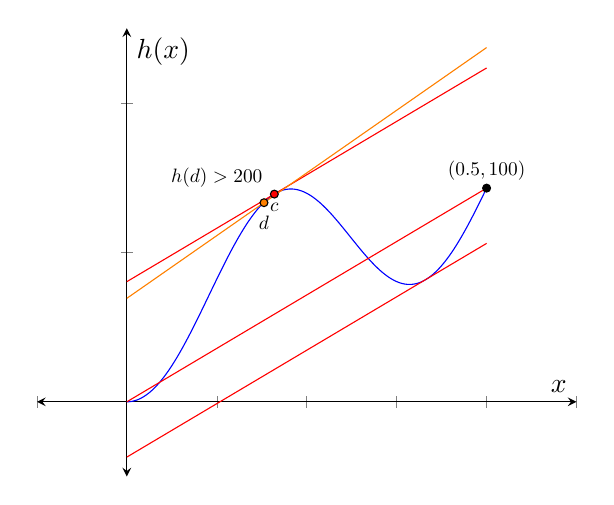
\begin{tikzpicture}[>=stealth]
        \begin{axis}[
            xmin=-1,xmax=5,
            ymin=-1,ymax=5,
            axis x line=middle,
            axis y line=middle,
            yticklabel=\empty,
            xticklabel=\empty,
            axis line style=<->,
            xlabel={$x$},
            ylabel={$h(x)$},
            ]
            \addplot[no marks,blue, -] expression[domain=0:4,samples=1000]
            {sin(deg((2*x)+4.458))+0.968+(0.5*x)};
            \addplot[no marks,red, -] expression[domain=0:4,samples=1000]
            {0.715*x};
            \addplot[no marks,red, -] expression[domain=0:4,samples=1000]
            {0.715*x+1.608};
            \addplot[no marks,red, -] expression[domain=0:4,samples=1000]
            {0.715*x-0.7398};

            \addplot[no marks,orange, -] expression[domain=0:4,samples=1000]
            {0.839*x+1.385};
            \node at (4,3.1) {\scalebox{0.7}{$(0.5,100)$}};
            \node at (1,3) {\scalebox{0.7}{$h(d) > 200$}};
            \node at (1.525,2.4) {\scalebox{0.7}{$d$}};
            \node at (1.64,2.6) {\scalebox{0.7}{$c$}};
            \node [draw, shape = circle, fill = black, minimum size = 0.1cm, inner sep=0pt] at (4,2.86){};
            \node [draw, shape = circle, fill = orange, minimum size = 0.1cm, inner sep=0pt] at (1.525,2.665){};
            \node [draw, shape = circle, fill = red, minimum size = 0.1cm, inner sep=0pt] at (1.64,2.78){};
        \end{axis}
        \end{tikzpicture}
    \end{center}
    Karena kecepatan total $h(d)$ melebihi $200$ km/jam. Maka salah satu mobil memiliki kecepatan tempuh 
    melebihi $100$ km/jam.

    $\therefore$ Telah ditunjukkan bahwa salah satu mobil memiliki kecepatan tempuh melebihi $100$ 
    km/jam.
\begin{center}
    \line(1,0){150}
\end{center}
    \item Karena kecepatan mobil $X$ tidak melebihi $90$ km/jam. Maka salah satu kemungkinannya 
    adalah mobil $X$ memiliki kecepatan $0$ km/jam. Pada kasus ini maka kecepatan maksimum mobil $Y$ 
    adalah $\geq 200$ km/jam (karena kedua mobil berpapasan setelah 30 menit). Karena mobil $Y$ juga 
    diasumsikan berangkat dari keadaan diam maka kecepatan sesaat mobil $Y$ berada diantara $0$ hingga 
    kecepatan maksimumnya. Dapat disimpulkan kecepatan sesaat mobil $Y$ selama perjalanan ada di interval 
    $[0, a]$ km/jam dimana $a \geq 200$.

    $\therefore$ Kecepatan sesaat mobil $Y$ selama perjalanan berada di antara $[0,a]$ km/jam dimana 
    $a \geq 200$.
\end{enumerate}

\end{enumerate}
\begin{center}
    \line(1,0){300}
\end{center}